\section{Articulation Points}
\begin{frame}
  \begin{center}
    {\bf Part III -- Articulation Vertices and Edges}
  \end{center}
\end{frame}

\begin{frame}
  \frametitle{Articulation Points and Bridges}
    \begin{block}{Definition: In a graph $G$}
      \begin{itemize}
      \item Vertex $v_i$ is an {\bf Articulation Point} if removing $v_i$ makes $G$ disconnected.
      \item Edge $e_{i,j}$ is a {\bf Bridge} if removing $e_{i,j}$ makes $G$ disconnected.
      \end{itemize}
    \end{block}
    \begin{center}
        \begin{tikzpicture}[scale=1.3,auto,swap]
          \node[vertex] (a) at (0,0) {};
          \node[vertex] (b) at (2,0) {};
          \node[red vertex] (c) at (0,2) {};
          \node[red vertex] (d) at (2,2) {};
          \node[red vertex] (e) at (3,1) {};
          \node[vertex] (f) at (4,0) {};
          \node[vertex] (g) at (4,2) {};
          \node[blue vertex] (h) at (3,3) {};
          \draw[edge] (a) to (b);
          \draw[edge] (a) to (c);
          \draw[edge] (c) to (d);
          \draw[edge] (d) to (b);
          \draw[red edge] (d) to (e);
          \draw[edge] (e) to (f);
          \draw[edge] (f) to (g);
          \draw[edge] (g) to (e);
          \draw[red edge] (c) to (h);
        \end{tikzpicture}
      \end{center}
\end{frame}

\begin{frame}
  \frametitle{Problems and Naive Algorithm}
  \begin{exampleblock}{Example Problems}
    \begin{itemize}
      \item Find vertices that can be removed from a graph to "break" it;
      \item Add extra edges to "reinforce" a graph;
      \item Measure the reliability of a network, etc;
    \end{itemize}
  \end{exampleblock}\medskip

  \begin{block}{Complete Search algorithm to find Articulation Points: $O(V\times(V+E)) = O(V^2+VE)$}
  \begin{enumerate}
    \item Run DFS/BFS, and count the number of CC in the graph;
    \item For each vertex $v_i$, remove $v_i$ and run DFS/BFS again;
    \item If the number of CC increases, $v_i$ is an articulation point;
  \end{enumerate}
  \end{block}
\end{frame}

\begin{frame}{Tarjan's DFS variant for Articulation point (O(V+E))}
  \begin{exampleblock}{Find Articulation Points/Bridges in a single DFS pass: $O(V+E)$}
    Main idea: Track loops to detect articulations:
    \begin{itemize}
    \item {\bf dfs\_num[i]}: visitation order from DFS;
    \item {\bf dfs\_low[i]}: lowest dfs\_num reachable from $v_i$;
    \end{itemize}\bigskip

    For neighbors $u,v$, if low[$v$] >= num[$u$], then $u$ is an articulation node (except root)\bigskip

    For neighbors $u,v$, if low[$v$] > num[$u$], $e_{u,v}$ is a bridge; (articulation edge)
  \end{exampleblock}
\end{frame}

% \begin{frame}{Tarjan's DFS variant for Articulation point (O(V+E))}
%
%   \begin{center}
%     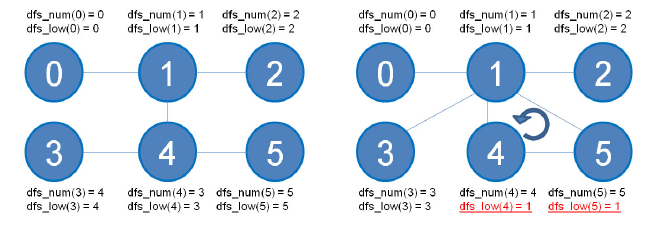
\includegraphics[width=0.9\textwidth]{../img/graph_articulation}
%   \end{center}
%   \ppagenote{Tarjan's attributes image from Competitive Programming 3}
% \end{frame}

\begin{frame}{Tarjan's Algorithm for Articulation Point}{Simulation}
  \begin{columns}
    \column{.45\textwidth}
    \begin{tikzpicture}[scale=1.3,auto,swap]
      \node[vertex] (a) at (0,0) {0};
      \node[vertex] (b) at (2,0) {1};
      \node[vertex] (c) at (0,2) {3};
      \node[vertex] (d) at (2,2) {2};
      \node[vertex] (e) at (3,1) {5};
      \node[vertex] (f) at (4,0) {6};
      \node[vertex] (g) at (4,2) {7};
      \node[vertex] (h) at (3,3) {4};
      \draw[edge] (a) to (b);
      \draw[edge] (a) to (c);
      \draw[edge] (c) to (d);
      \draw[edge] (d) to (b);
      \draw[edge] (d) to (e);
      \draw[edge] (e) to (f);
      \draw[edge] (f) to (g);
      \draw[edge] (g) to (e);
      \draw[edge] (c) to (h);
    \end{tikzpicture}
    \column{.55\textwidth}
    First, use DFS to calculate dfs\_num and dfs\_low\\
    Then compare neighbors to check articulation node/edge.
    \begin{itemize}
      \item dfs\_num: 0; dfs\_low: 0
      \item dfs\_num: 1; dfs\_low: 0
      \item dfs\_num: 2; dfs\_low: 0
      \item dfs\_num: 3; dfs\_low: 0
      \item dfs\_num: 4; dfs\_low: 4
      \item dfs\_num: 5; dfs\_low: 5
      \item dfs\_num: 6; dfs\_low: 5
      \item dfs\_num: 7; dfs\_low: 5
    \end{itemize}
  \end{columns}
\end{frame}

\begin{frame}[fragile]{Tarjan's Algorithm for Articulation Point}
  
{\smaller
  \begin{exampleblock}{}
\begin{verbatim}
void articulation(u){
   dfs_num[u] = dfs_low[u] = IterationCounter++; // update num[u], init low[u]
   for (int i = 0; i < AdjList[u].size(); i++){  // Do DFS on each edge from u
      v = AdjList[u][i];
      if (dfs_num[v.first] == UNVISITED) {       // DFS tree edge
         dfs_parent[v.first] = u;                // store parent
         if (u == 0) rootTreeEdge++;             // special case for root vertex
         articulation(v.first);                  // visit next vertex

         // After we finish the DFS from u, we check if u is articulation.
         if (dfs_low[v.first] >= dfs_num[u])
            articulation_vertex[u] = true;       // u is articulation
         dfs_low[u] = min(dfs_low[u],dfs_low[v.first])
      }
      else if (v.first != dfs_parent[u])         // found a cycle edge
         dfs_low[u] = min(dfs_low[u],dfs_num[v.first]);
}  }
\end{verbatim}
  \end{exampleblock}}
\end{frame}

\subsection{Strongly Connected Components}

\begin{frame}{Strongly Connected Components}
    \begin{block}{Definition}
      Given a {\bf directed} graph $G(V,E)$, a {\bf Strongly Connected Component (SCC)} is a subset of vertices $V_1$ where for every pair of vertices $v_i, v_j \in V_1$, there is both a path $v_i \to v_j$ and a path $v_j \to v_i$.
    \end{block}


\begin{columns}[t]
    \column{0.5\textwidth}
    \begin{exampleblock}{One Connected Component (undirected)}
      \vspace{0.1cm}
      \begin{center}
        \begin{tikzpicture}[scale=1.1,auto,swap]
          \node[vertex] (a) at (0,0) {};
          \node[vertex] (b) at (1,0) {};
          \node[vertex] (c) at (2,0) {};
          \node[vertex] (d) at (1,1) {};
          \node[vertex] (e) at (3,0) {};
          \node[vertex] (f) at (4,0) {};
          \node[vertex] (g) at (4,1) {};
          \node[vertex] (h) at (3,1) {};
          \draw[edge] (a) to (b);
          \draw[edge] (b) to (c);
          \draw[edge] (c) to (d);
          \draw[edge] (d) to (b);
          \draw[edge] (c) to (e);
          \draw[edge] (e) to (f);
          \draw[edge] (f) to (g);
          \draw[edge] (g) to (h);
          \draw[edge] (h) to (e);
        \end{tikzpicture}
      \end{center}
      \vspace{0.1cm}
    \end{exampleblock}
    \column{0.5\textwidth}
    \begin{exampleblock}{Three SCC (directed)}
      \vspace{0.1cm}
      \begin{center}
        \begin{tikzpicture}[scale=1.1,auto,swap]
          \tikzset{edge/.style = {->,>=latex'}}
          \node[vertex] (a) at (0,0) {};
          \node[blue vertex] (b) at (1,0) {};
          \node[blue vertex] (c) at (2,0) {};
          \node[blue vertex] (d) at (1,1) {};
          \node[red vertex] (e) at (3,0) {};
          \node[red vertex] (f) at (4,0) {};
          \node[red vertex] (g) at (4,1) {};
          \node[red vertex] (h) at (3,1) {};
          \draw[edge] (a) to (b);
          \draw[edge] (b) to (c);
          \draw[edge] (c) to (d);
          \draw[edge] (d) to (b);
          \draw[edge] (c) to (e);
          \draw[edge] (e) to (f);
          \draw[edge] (f) to (g);
          \draw[edge] (g) to (h);
          \draw[edge] (h) to (e);
        \end{tikzpicture}
      \end{center}
      \vspace{0.1cm}
    \end{exampleblock}
  \end{columns}
\end{frame}

\begin{frame}{Algorithm for Finding SCCs}

  We can modify Tarjan's algorithm (for articulation points and bridges) to find Strongly Connected Components:\bigskip

  \begin{block}{}
  \begin{itemize}
    \item Every time we visit a new vertex $u$, we put $u$ in a stack $S$;
    \item Only update dfs\_low for vertices with the "visited" flag = 1;
    \item After visiting all edges of $u$, check if "dfs\_num[$u$] == dfs\_low[$u$]";
    \item If the condition is true, $u$ is the root of a new SCC.
    \item Pop all vertices in $S$ until (and including) $u$;
    \item Add all popped vertices to the SCC.
  \end{itemize}
  \end{block}
\end{frame}

\begin{frame}[fragile]{Algorithm for Finding SCCs}{Do this simulation yourself!}
  \begin{center}
    \begin{tikzpicture}[scale=1.1,auto,swap]
      \tikzset{edge/.style = {->,>=latex'}}
      \node[vertex] (a) at (0,0) {0};
      \node[vertex] (b) at (1,0) {1};
      \node[vertex] (c) at (2,0) {2};
      \node[vertex] (d) at (1,1) {3};
      \node[vertex] (e) at (3,0) {4};
      \node[vertex] (f) at (4,0) {5};
      \node[vertex] (g) at (4,1) {6};
      \node[vertex] (h) at (3,1) {7};
      \draw[edge] (a) to (b);
      \draw[edge] (b) to (c);
      \draw[edge] (c) to (d);
      \draw[edge] (d) to (b);
      \draw[edge] (c) to (e);
      \draw[edge] (e) to (f);
      \draw[edge] (f) to (g);
      \draw[edge] (g) to (h);
      \draw[edge] (h) to (e);
    \end{tikzpicture}
  \end{center}
  \bigskip
  {\bf SCC Stack:}\bigskip

\begin{verbatim}
          0   1   2   3   4   5   6   7

dfs_low

dfs_num
\end{verbatim}

\end{frame}

%%%%%%%%%%%%%%%%%%%%%%%%%%%%%%%%%%%%%%%%%%%%%%%
